\import{./tikz-arrays/}{img-examples}
\import{./tikz-arrays/}{component-tree}
\import{./tikz-arrays/}{compact-tree}
\import{./tikz-arrays/}{tree-of-shapes}



\newarray\imgExamplePruned
\readarray{imgExamplePruned}{%
0 & 0 & 0 & 0 & 0 & 0 & 0 &
0 & 4 & 4 & 4 & 7 & 7 & 7 &
0 & 4 & 4 & 4 & 7 & 4 & 7 &
0 & 4 & 4 & 4 & 7 & 4 & 7 &
0 & 4 & 4 & 4 & 7 & 4 & 7 &
0 & 4 & 4 & 4 & 7 & 7 & 7 &
0 & 0 & 0 & 0 & 0 & 0 & 0}


\newarray\imgExampleNodeA
\readarray{imgExampleNodeA}{%
0 & 0 & 0 & 0 & 0 & 0 & 0 &
0 & 0 & 0 & 0 & 1 & 1 & 1 &
0 & 0 & 0 & 0 & 1 & 0 & 1 &
0 & 0 & 0 & 0 & 1 & 0 & 1 &
0 & 0 & 0 & 0 & 1 & 0 & 1 &
0 & 0 & 0 & 0 & 1 & 1 & 1 &
0 & 0 & 0 & 0 & 0 & 0 & 0 &
}

\newsavebox\imgExampleNodeABox
\begin{lrbox}{\imgExampleNodeABox}
   \begin{tikzpicture}[scale=0.15] \drawBinaryImage{7}{7}{imgExampleNodeA} \end{tikzpicture}
\end{lrbox}

\newarray\imgExampleNodeB
\readarray{imgExampleNodeB}{%
0 & 0 & 0 & 0 & 0 & 0 & 0 &
0 & 0 & 0 & 0 & 0 & 0 & 0 &
0 & 0 & 0 & 0 & 0 & 0 & 0 &
0 & 0 & 0 & 0 & 0 & 0 & 0 &
0 & 0 & 0 & 0 & 0 & 0 & 0 &
0 & 1 & 1 & 0 & 0 & 0 & 0 &
0 & 0 & 0 & 0 & 0 & 0 & 0 &
}

\newsavebox\imgExampleNodeBBox
\begin{lrbox}{\imgExampleNodeBBox}
   \begin{tikzpicture}[scale=0.15] \drawBinaryImage{7}{7}{imgExampleNodeB} \end{tikzpicture}
\end{lrbox}

\newarray\imgExampleNodeC
\readarray{imgExampleNodeC}{%
0 & 0 & 0 & 0 & 0 & 0 & 0 &
0 & 0 & 0 & 0 & 0 & 0 & 0 &
0 & 1 & 1 & 0 & 0 & 0 & 0 &
0 & 1 & 0 & 0 & 0 & 0 & 0 &
0 & 0 & 0 & 0 & 0 & 0 & 0 &
0 & 0 & 0 & 0 & 0 & 0 & 0 &
0 & 0 & 0 & 0 & 0 & 0 & 0 &
}

\newsavebox\imgExampleNodeCBox
\begin{lrbox}{\imgExampleNodeCBox}
   \begin{tikzpicture}[scale=0.15]\drawBinaryImage{7}{7}{imgExampleNodeC}\end{tikzpicture}
\end{lrbox}

\newarray\imgExampleNodeD
\readarray{imgExampleNodeD}{%
0 & 0 & 0 & 0 & 0 & 0 & 0 &
0 & 1 & 1 & 1 & 1 & 1 & 1 &
0 & 1 & 1 & 1 & 1 & 1 & 1 &
0 & 1 & 1 & 1 & 1 & 1 & 1 &
0 & 1 & 1 & 1 & 1 & 1 & 1 &
0 & 1 & 1 & 1 & 1 & 1 & 1 &
0 & 0 & 0 & 0 & 0 & 0 & 0 &
}

\newsavebox\imgExampleNodeDBox
\begin{lrbox}{\imgExampleNodeDBox}
   \begin{tikzpicture}[scale=0.15] \drawBinaryImage{7}{7}{imgExampleNodeD} \end{tikzpicture}
\end{lrbox}

\newarray\imgExampleNodeR
\readarray{imgExampleNodeR}{%
1 & 1 & 1 & 1 & 1 & 1 & 1 &
1 & 1 & 1 & 1 & 1 & 1 & 1 &
1 & 1 & 1 & 1 & 1 & 1 & 1 &
1 & 1 & 1 & 1 & 1 & 1 & 1 &
1 & 1 & 1 & 1 & 1 & 1 & 1 &
1 & 1 & 1 & 1 & 1 & 1 & 1 &
1 & 1 & 1 & 1 & 1 & 1 & 1 &
}

\newsavebox\imgExampleNodeRBox
\begin{lrbox}{\imgExampleNodeRBox}
   \begin{tikzpicture}[scale=0.15] \drawBinaryImage{7}{7}{imgExampleNodeR} \end{tikzpicture}
\end{lrbox}



% -------------- Bit-Quads counting repetition  -------------------%
\newarray\QOneExample
\readarray{QOneExample}{%
0 & 1 &
0 & 0}

\newarray\QTwoExample
\readarray{QTwoExample}{%
0 & 1 &
0 & 1}

\newsavebox\imgExampleNodeBWithQOneBox
\begin{lrbox}{\imgExampleNodeBWithQOneBox}
  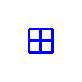
\begin{tikzpicture}[scale=0.15]
    \drawBinaryImage{7}{7}{imgExampleNodeB}
    \draw[blue, line width=1pt] (0,0) grid (2,2);
  \end{tikzpicture}
\end{lrbox}

\newsavebox\imgExampleNodeCWithQTwoBox
\begin{lrbox}{\imgExampleNodeCWithQTwoBox}
  
\begin{tikzpicture}[scale=0.15]
    \drawBinaryImage{7}{7}{imgExampleNodeC}
    \draw[red, line width=1pt] (0,3) grid (2,5);
  \end{tikzpicture}
\end{lrbox}

\newsavebox\imgExampleNodeDWithQuadsBox
\begin{lrbox}{\imgExampleNodeDWithQuadsBox}
  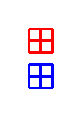
\begin{tikzpicture}[scale=0.15]
    \drawBinaryImage{7}{7}{imgExampleNodeD}
    \draw[blue, line width=1pt] (0,0) grid (2,2);
    \draw[red, line width=1pt] (0,3) grid (2,5);
  \end{tikzpicture}
\end{lrbox}


\newarray\binaryImgExample
\readarray{binaryImgExample}{%
0 & 0 & 0 & 0 & 0 & 0 & 0 &
0 & 0 & 0 & 0 & 1 & 1 & 1 &
0 & 1 & 1 & 0 & 1 & 0 & 1 &
0 & 1 & 0 & 0 & 1 & 0 & 1 &
0 & 0 & 0 & 0 & 1 & 0 & 1 &
0 & 1 & 1 & 0 & 1 & 1 & 1 &
0 & 0 & 0 & 0 & 0 & 0 & 0}


\newarray\imgCCExample
\readarray{imgCCExample}{%
0 & 0 & 0 & 1 &
0 & 1 & 1 & 1 &
1 & 0 & 0 & 1 &
1 & 0 & 0 & 0}

\newarray\firstLevelSet
\readarray{firstLevelSet}{%
1 & 1 & 1 & 1 & 1 & 1 & 1 &
1 & 1 & 1 & 1 & 1 & 1 & 1 &
1 & 1 & 1 & 1 & 1 & 1 & 1 &
1 & 1 & 1 & 1 & 1 & 1 & 1 &
1 & 1 & 1 & 1 & 1 & 1 & 1 &
1 & 1 & 1 & 1 & 1 & 1 & 1 &
1 & 1 & 1 & 1 & 1 & 1 & 1}

\newarray\lowerLevelSetFour
\readarray{lowerLevelSetFour}{%
1 & 1 & 1 & 1 & 1 & 1 & 1 &
1 & 1 & 1 & 1 & 0 & 0 & 0 &
1 & 0 & 0 & 1 & 0 & 1 & 0 &
1 & 0 & 1 & 1 & 0 & 1 & 0 &
1 & 1 & 1 & 1 & 0 & 1 & 0 &
1 & 0 & 0 & 1 & 0 & 0 & 0 &
1 & 1 & 1 & 1 & 1 & 1 & 1}

\newarray\upperLevelSetFour
\readarray{upperLevelSetFour}{%
0 & 0 & 0 & 0 & 0 & 0 & 0 &
0 & 1 & 1 & 1 & 1 & 1 & 1 &
0 & 1 & 1 & 1 & 1 & 1 & 1 &
0 & 1 & 1 & 1 & 1 & 1 & 1 &
0 & 1 & 1 & 1 & 1 & 1 & 1 &
0 & 1 & 1 & 1 & 1 & 1 & 1 &
0 & 0 & 0 & 0 & 0 & 0 & 0}

\newarray\lowerLevelSetZero
\readarray{lowerLevelSetZero}{%
1 & 1 & 1 & 1 & 1 & 1 & 1 &
1 & 0 & 0 & 0 & 0 & 0 & 0 &
1 & 0 & 0 & 0 & 0 & 0 & 0 &
1 & 0 & 0 & 0 & 0 & 0 & 0 &
1 & 0 & 0 & 0 & 0 & 0 & 0 &
1 & 0 & 0 & 0 & 0 & 0 & 0 &
1 & 1 & 1 & 1 & 1 & 1 & 1}

\newarray\upperLevelSetSeven
\readarray{upperLevelSetSeven}{%
0 & 0 & 0 & 0 & 0 & 0 & 0 &
0 & 0 & 0 & 0 & 1 & 1 & 1 &
0 & 1 & 1 & 0 & 1 & 0 & 1 &
0 & 1 & 0 & 0 & 1 & 0 & 1 &
0 & 0 & 0 & 0 & 1 & 0 & 1 &
0 & 1 & 1 & 0 & 1 & 1 & 1 &
0 & 0 & 0 & 0 & 0 & 0 & 0}



%--------------- Arvore de componentes L(f)  -----------------------------------------%
\newarray\imgExampleLCTNodeA
\readarray{imgExampleLCTNodeA}{%
1 & 1 & 1 & 1 & 1 & 1 & 1 &
1 & 0 & 0 & 0 & 0 & 0 & 0 &
1 & 0 & 0 & 0 & 0 & 0 & 0 &
1 & 0 & 0 & 0 & 0 & 0 & 0 &
1 & 0 & 0 & 0 & 0 & 0 & 0 &
1 & 0 & 0 & 0 & 0 & 0 & 0 &
1 & 1 & 1 & 1 & 1 & 1 & 1 &
}

\newsavebox\imgExampleLCTNodeABox
\begin{lrbox}{\imgExampleLCTNodeABox}
   \begin{tikzpicture}[scale=0.15]\drawBinaryImage{7}{7}{imgExampleLCTNodeA}\end{tikzpicture}
\end{lrbox}

\newarray\imgExampleLCTNodeB
\readarray{imgExampleLCTNodeB}{%
1 & 1 & 1 & 1 & 1 & 1 & 1 &
1 & 1 & 1 & 1 & 0 & 0 & 0 &
1 & 0 & 0 & 1 & 0 & 0 & 0 &
1 & 0 & 1 & 1 & 0 & 0 & 0 &
1 & 1 & 1 & 1 & 0 & 0 & 0 &
1 & 0 & 0 & 1 & 0 & 0 & 0 &
1 & 1 & 1 & 1 & 1 & 1 & 1 &
}

\newsavebox\imgExampleLCTNodeBBox
\begin{lrbox}{\imgExampleLCTNodeBBox}
   \begin{tikzpicture}[scale=0.15]\drawBinaryImage{7}{7}{imgExampleLCTNodeB}\end{tikzpicture}
\end{lrbox}

\newarray\imgExampleLCTNodeC
\readarray{imgExampleLCTNodeC}{%
0 & 0 & 0 & 0 & 0 & 0 & 0 &
0 & 0 & 0 & 0 & 0 & 0 & 0 &
0 & 0 & 0 & 0 & 0 & 1 & 0 &
0 & 0 & 0 & 0 & 0 & 1 & 0 &
0 & 0 & 0 & 0 & 0 & 1 & 0 &
0 & 0 & 0 & 0 & 0 & 0 & 0 &
0 & 0 & 0 & 0 & 0 & 0 & 0 &
}

\newsavebox\imgExampleLCTNodeCBox
\begin{lrbox}{\imgExampleLCTNodeCBox}
   \begin{tikzpicture}[scale=0.15]\drawBinaryImage{7}{7}{imgExampleLCTNodeC}\end{tikzpicture}
\end{lrbox}


% Examples of max-tree and min-tree respectively
\newarray\imgMaxTreeRNode
\readarray{imgMaxTreeRNode}{%
3 & 3 & 3 & 3 & 3 & 3 & 3 &
3 & 1 & 1 & 1 & 1 & 1 & 1 &
3 & 1 & 1 & 1 & 1 & 1 & 1 &
3 & 1 & 1 & 1 & 1 & 1 & 1 &
3 & 1 & 1 & 1 & 1 & 1 & 1 &
3 & 1 & 1 & 1 & 1 & 1 & 1 &
3 & 3 & 3 & 3 & 3 & 3 & 3}

\newsavebox\imgMaxTreeRNodeBox
\begin{lrbox}{\imgMaxTreeRNodeBox}
  \begin{tikzpicture}[scale=0.15]\drawBinaryImage{7}{7}{imgMaxTreeRNode}\end{tikzpicture}
\end{lrbox}

\newarray\imgMaxTreeDNode
\readarray{imgMaxTreeDNode}{%
0 & 0 & 0 & 0 & 0 & 0 & 0 &
0 & 3 & 3 & 3 & 1 & 1 & 1 &
0 & 1 & 1 & 3 & 1 & 3 & 1 &
0 & 1 & 3 & 3 & 1 & 3 & 1 &
0 & 3 & 3 & 3 & 1 & 3 & 1 &
0 & 1 & 1 & 3 & 1 & 1 & 1 &
0 & 0 & 0 & 0 & 0 & 0 & 0}

\newsavebox\imgMaxTreeDNodeBox
\begin{lrbox}{\imgMaxTreeDNodeBox}
  \begin{tikzpicture}[scale=0.15]\drawBinaryImage{7}{7}{imgMaxTreeDNode}\end{tikzpicture}
\end{lrbox}

\newarray\imgMaxTreeANode
\readarray{imgMaxTreeANode}{%
0 & 0 & 0 & 0 & 0 & 0 & 0 &
0 & 0 & 0 & 0 & 3 & 3 & 3 &
0 & 0 & 0 & 0 & 3 & 0 & 3 &
0 & 0 & 0 & 0 & 3 & 0 & 3 &
0 & 0 & 0 & 0 & 3 & 0 & 3 &
0 & 0 & 0 & 0 & 3 & 3 & 3 &
0 & 0 & 0 & 0 & 0 & 0 & 0}

\newsavebox\imgMaxTreeANodeBox
\begin{lrbox}{\imgMaxTreeANodeBox}
  \begin{tikzpicture}[scale=0.15]\drawBinaryImage{7}{7}{imgMaxTreeANode}\end{tikzpicture}
\end{lrbox}

\newarray\imgMaxTreeBNode
\readarray{imgMaxTreeBNode}{%
0 & 0 & 0 & 0 & 0 & 0 & 0 &
0 & 0 & 0 & 0 & 0 & 0 & 0 &
0 & 0 & 0 & 0 & 0 & 0 & 0 &
0 & 0 & 0 & 0 & 0 & 0 & 0 &
0 & 0 & 0 & 0 & 0 & 0 & 0 &
0 & 3 & 3 & 0 & 0 & 0 & 0 &
0 & 0 & 0 & 0 & 0 & 0 & 0}

\newsavebox\imgMaxTreeBNodeBox
\begin{lrbox}{\imgMaxTreeBNodeBox}
  \begin{tikzpicture}[scale=0.15]\drawBinaryImage{7}{7}{imgMaxTreeBNode}\end{tikzpicture}
\end{lrbox}

\newarray\imgMaxTreeCNode
\readarray{imgMaxTreeCNode}{%
0 & 0 & 0 & 0 & 0 & 0 & 0 &
0 & 0 & 0 & 0 & 0 & 0 & 0 &
0 & 3 & 3 & 0 & 0 & 0 & 0 &
0 & 3 & 0 & 0 & 0 & 0 & 0 &
0 & 0 & 0 & 0 & 0 & 0 & 0 &
0 & 0 & 0 & 0 & 0 & 0 & 0 &
0 & 0 & 0 & 0 & 0 & 0 & 0}

\newsavebox\imgMaxTreeCNodeBox
\begin{lrbox}{\imgMaxTreeCNodeBox}
  \begin{tikzpicture}[scale=0.15]\drawBinaryImage{7}{7}{imgMaxTreeCNode}\end{tikzpicture}
\end{lrbox}

\newarray\imgMinTreeRNode
\readarray{imgMinTreeRNode}{%
1 & 1 & 1 & 1 & 1 & 1 & 1 &
1 & 1 & 1 & 1 & 3 & 3 & 3 &
1 & 3 & 3 & 1 & 3 & 1 & 3 &
1 & 3 & 1 & 1 & 3 & 1 & 3 &
1 & 1 & 1 & 1 & 3 & 1 & 3 &
1 & 3 & 3 & 1 & 3 & 3 & 3 &
1 & 1 & 1 & 1 & 1 & 1 & 1}

\newsavebox\imgMinTreeRNodeBox
\begin{lrbox}{\imgMinTreeRNodeBox}
  \begin{tikzpicture}[scale=0.15]\drawBinaryImage{7}{7}{imgMinTreeRNode}\end{tikzpicture}
\end{lrbox}

\newarray\imgMinTreeBNode
\readarray{imgMinTreeBNode}{%
1 & 1 & 1 & 1 & 1 & 1 & 1 &
1 & 3 & 3 & 3 & 0 & 0 & 0 &
1 & 0 & 0 & 3 & 0 & 0 & 0 &
1 & 0 & 3 & 3 & 0 & 0 & 0 &
1 & 3 & 3 & 3 & 0 & 0 & 0 &
1 & 0 & 0 & 3 & 0 & 0 & 0 &
1 & 1 & 1 & 1 & 1 & 1 & 1}

\newsavebox\imgMinTreeBNodeBox
\begin{lrbox}{\imgMinTreeBNodeBox}
  \begin{tikzpicture}[scale=0.15]\drawBinaryImage{7}{7}{imgMinTreeBNode}\end{tikzpicture}
\end{lrbox}


\newarray\imgMinTreeCNode
\readarray{imgMinTreeCNode}{%
0 & 0 & 0 & 0 & 0 & 0 & 0 &
0 & 0 & 0 & 0 & 0 & 0 & 0 &
0 & 0 & 0 & 0 & 0 & 3 & 0 &
0 & 0 & 0 & 0 & 0 & 3 & 0 &
0 & 0 & 0 & 0 & 0 & 3 & 0 &
0 & 0 & 0 & 0 & 0 & 0 & 0 &
0 & 0 & 0 & 0 & 0 & 0 & 0}

\newsavebox\imgMinTreeCNodeBox
\begin{lrbox}{\imgMinTreeCNodeBox}
  \begin{tikzpicture}[scale=0.15]\drawBinaryImage{7}{7}{imgMinTreeCNode}\end{tikzpicture}
\end{lrbox}

\newarray\imgMinTreeANode
\readarray{imgMinTreeANode}{%
3 & 3 & 3 & 3 & 3 & 3 & 3 &
3 & 0 & 0 & 0 & 0 & 0 & 0 &
3 & 0 & 0 & 0 & 0 & 0 & 0 &
3 & 0 & 0 & 0 & 0 & 0 & 0 &
3 & 0 & 0 & 0 & 0 & 0 & 0 &
3 & 0 & 0 & 0 & 0 & 0 & 0 &
3 & 3 & 3 & 3 & 3 & 3 & 3}

\newsavebox\imgMinTreeANodeBox
\begin{lrbox}{\imgMinTreeANodeBox}
  \begin{tikzpicture}[scale=0.15]\drawBinaryImage{7}{7}{imgMinTreeANode}\end{tikzpicture}
\end{lrbox}

%% ----------------------- Example area calculation ------------------------------------------
\newarray\imgMaxTreeRNodeOnlyRed
\readarray{imgMaxTreeRNodeOnlyRed}{%
3 & 3 & 3 & 3 & 3 & 3 & 3 &
3 & 1 & 1 & 1 & 1 & 1 & 1 &
3 & 1 & 1 & 1 & 1 & 1 & 1 &
3 & 1 & 1 & 1 & 1 & 1 & 1 &
3 & 1 & 1 & 1 & 1 & 1 & 1 &
3 & 1 & 1 & 1 & 1 & 1 & 1 &
3 & 3 & 3 & 3 & 3 & 3 & 3}

\newsavebox\imgMaxTreeRNodeOnlyRedBox
\begin{lrbox}{\imgMaxTreeRNodeOnlyRedBox}
  \begin{tikzpicture}[scale=0.15]\drawBinaryImage{7}{7}{imgMaxTreeRNodeOnlyRed}\end{tikzpicture}
\end{lrbox}

\newsavebox\imgMaxTreeRNodeTransformation
\begin{lrbox}{\imgMaxTreeRNodeTransformation}
	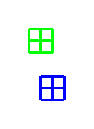
\begin{tikzpicture}[scale=0.15]
		\drawBinaryImage{7}{7}{imgMaxTreeRNodeOnlyRed}
		\draw[green, line width=1pt] (4,6) grid (6,4);
		\draw[blue, line width=1pt] (5,2) grid (7,0);
	\end{tikzpicture}
\end{lrbox}

\newarray\imgMaxTreeDNodeOnlyRed
\readarray{imgMaxTreeDNodeOnlyRed}{%
0 & 0 & 0 & 0 & 0 & 0 & 0 &
0 & 3 & 3 & 3 & 1 & 1 & 1 &
0 & 1 & 1 & 3 & 1 & 3 & 1 &
0 & 1 & 3 & 3 & 1 & 3 & 1 &
0 & 3 & 3 & 3 & 1 & 3 & 1 &
0 & 1 & 1 & 3 & 1 & 1 & 1 &
0 & 0 & 0 & 0 & 0 & 0 & 0}

\newsavebox\imgMaxTreeDNodeOnlyRedBox
\begin{lrbox}{\imgMaxTreeDNodeOnlyRedBox}
  \begin{tikzpicture}[scale=0.15]\drawBinaryImage{7}{7}{imgMaxTreeDNodeOnlyRed}\end{tikzpicture}
\end{lrbox}

\newarray\imgMaxTreeANodeOnlyRed
\readarray{imgMaxTreeANodeOnlyRed}{%
0 & 0 & 0 & 0 & 0 & 0 & 0 &
0 & 0 & 0 & 0 & 3 & 3 & 3 &
0 & 0 & 0 & 0 & 3 & 0 & 3 &
0 & 0 & 0 & 0 & 3 & 0 & 3 &
0 & 0 & 0 & 0 & 3 & 0 & 3 &
0 & 0 & 0 & 0 & 3 & 3 & 3 &
0 & 0 & 0 & 0 & 0 & 0 & 0}

\newsavebox\imgMaxTreeANodeOnlyRedBox
\begin{lrbox}{\imgMaxTreeANodeOnlyRedBox}
  \begin{tikzpicture}[scale=0.15]\drawBinaryImage{7}{7}{imgMaxTreeANodeOnlyRed}\end{tikzpicture}
\end{lrbox}

\newarray\imgMaxTreeBNodeOnlyRed
\readarray{imgMaxTreeBNodeOnlyRed}{%
0 & 0 & 0 & 0 & 0 & 0 & 0 &
0 & 0 & 0 & 0 & 0 & 0 & 0 &
0 & 0 & 0 & 0 & 0 & 0 & 0 &
0 & 0 & 0 & 0 & 0 & 0 & 0 &
0 & 0 & 0 & 0 & 0 & 0 & 0 &
0 & 3 & 3 & 0 & 0 & 0 & 0 &
0 & 0 & 0 & 0 & 0 & 0 & 0}

\newsavebox\imgMaxTreeBNodeOnlyRedBox
\begin{lrbox}{\imgMaxTreeBNodeOnlyRedBox}
  \begin{tikzpicture}[scale=0.15]\drawBinaryImage{7}{7}{imgMaxTreeBNodeOnlyRed}\end{tikzpicture}
\end{lrbox}

\newarray\imgMaxTreeCNodeOnlyRed
\readarray{imgMaxTreeCNodeOnlyRed}{%
0 & 0 & 0 & 0 & 0 & 0 & 0 &
0 & 0 & 0 & 0 & 0 & 0 & 0 &
0 & 3 & 3 & 0 & 0 & 0 & 0 &
0 & 3 & 0 & 0 & 0 & 0 & 0 &
0 & 0 & 0 & 0 & 0 & 0 & 0 &
0 & 0 & 0 & 0 & 0 & 0 & 0 &
0 & 0 & 0 & 0 & 0 & 0 & 0}

\newsavebox\imgMaxTreeCNodeOnlyRedBox
\begin{lrbox}{\imgMaxTreeCNodeOnlyRedBox}
  \begin{tikzpicture}[scale=0.15]\drawBinaryImage{7}{7}{imgMaxTreeCNodeOnlyRed}\end{tikzpicture}
\end{lrbox}

\newarray\imgMinTreeRNodeOnlyRed
\readarray{imgMinTreeRNodeOnlyRed}{%
1 & 1 & 1 & 1 & 1 & 1 & 1 &
1 & 1 & 1 & 1 & 3 & 3 & 3 &
1 & 3 & 3 & 1 & 3 & 1 & 3 &
1 & 3 & 1 & 1 & 3 & 1 & 3 &
1 & 1 & 1 & 1 & 3 & 1 & 3 &
1 & 3 & 3 & 1 & 3 & 3 & 3 &
1 & 1 & 1 & 1 & 1 & 1 & 1}

\newsavebox\imgMinTreeRNodeOnlyRedBox
\begin{lrbox}{\imgMinTreeRNodeOnlyRedBox}
  \begin{tikzpicture}[scale=0.15]\drawBinaryImage{7}{7}{imgMinTreeRNodeOnlyRed}\end{tikzpicture}
\end{lrbox}

\newarray\imgMinTreeBNodeOnlyRed
\readarray{imgMinTreeBNodeOnlyRed}{%
1 & 1 & 1 & 1 & 1 & 1 & 1 &
1 & 3 & 3 & 3 & 0 & 0 & 0 &
1 & 0 & 0 & 3 & 0 & 0 & 0 &
1 & 0 & 3 & 3 & 0 & 0 & 0 &
1 & 3 & 3 & 3 & 0 & 0 & 0 &
1 & 0 & 0 & 3 & 0 & 0 & 0 &
1 & 1 & 1 & 1 & 1 & 1 & 1}

\newsavebox\imgMinTreeBNodeOnlyRedBox
\begin{lrbox}{\imgMinTreeBNodeOnlyRedBox}
  \begin{tikzpicture}[scale=0.15]\drawBinaryImage{7}{7}{imgMinTreeBNodeOnlyRed}\end{tikzpicture}
\end{lrbox}


\newarray\imgMinTreeCNodeOnlyRed
\readarray{imgMinTreeCNodeOnlyRed}{%
0 & 0 & 0 & 0 & 0 & 0 & 0 &
0 & 0 & 0 & 0 & 0 & 0 & 0 &
0 & 0 & 0 & 0 & 0 & 3 & 0 &
0 & 0 & 0 & 0 & 0 & 3 & 0 &
0 & 0 & 0 & 0 & 0 & 3 & 0 &
0 & 0 & 0 & 0 & 0 & 0 & 0 &
0 & 0 & 0 & 0 & 0 & 0 & 0}

\newsavebox\imgMinTreeCNodeOnlyRedBox
\begin{lrbox}{\imgMinTreeCNodeOnlyRedBox}
  \begin{tikzpicture}[scale=0.15]\drawBinaryImage{7}{7}{imgMinTreeCNodeOnlyRed}\end{tikzpicture}
\end{lrbox}

\newarray\imgMinTreeANodeOnlyRed
\readarray{imgMinTreeANodeOnlyRed}{%
3 & 3 & 3 & 3 & 3 & 3 & 3 &
3 & 0 & 0 & 0 & 0 & 0 & 0 &
3 & 0 & 0 & 0 & 0 & 0 & 0 &
3 & 0 & 0 & 0 & 0 & 0 & 0 &
3 & 0 & 0 & 0 & 0 & 0 & 0 &
3 & 0 & 0 & 0 & 0 & 0 & 0 &
3 & 3 & 3 & 3 & 3 & 3 & 3}

\newsavebox\imgMinTreeANodeOnlyRedBox
\begin{lrbox}{\imgMinTreeANodeOnlyRedBox}
  \begin{tikzpicture}[scale=0.15]\drawBinaryImage{7}{7}{imgMinTreeANodeOnlyRed}\end{tikzpicture}
\end{lrbox}

%countB Binary patterns Example 

\newarray\patternExampleCountB
\readarray{patternExampleCountB}{%
1 & 0 &
1 & 1}

\newarray\patternDashExampleCountB
\readarray{patternDashExampleCountB}{%
0 & 1 &
1 & 1}

\newarray\patternDashExampleCountBInterImage
\readarray{patternDashExampleCountBInterImage}{%
0 & 1 &
0 & 1}

\newarray\patternExampleCountG
\readarray{patternExampleCountG}{%
7 & 4 &
7 & 7}

\newarray\patternDashExampleCountG
\readarray{patternDashExampleCountG}{%
4 & 7 &
4 & 7}

\newarray\patternDashDashExampleCountG
\readarray{patternDashDashExampleCountG}{%
0 & 0 &
7 & 7}


%countBR patterns Example
\newarray\patternExampleCountBR
\readarray{patternExampleCountBR}{%
0 & 0 &
1 & 0}

\newarray\patternDashExampleCountBR
\readarray{patternDashExampleCountBR}{%
1 & 0 &
0 & 0}

% Draw Transformation Rects %
\newsavebox\imgMaxTreeANodeOnlyRedTransformationBox
\begin{lrbox}{\imgMaxTreeANodeOnlyRedTransformationBox}
  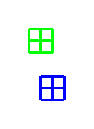
\begin{tikzpicture}[scale=0.15]
    \drawBinaryImage{7}{7}{imgMaxTreeANodeOnlyRed}
    \draw[green, line width=1pt] (4,6) grid (6,4);
    \draw[blue, line width=1pt] (5,2) grid (7,0);
  \end{tikzpicture}
\end{lrbox}

\newsavebox\imgMaxTreeDNodeOnlyRedTransformationBox
\begin{lrbox}{\imgMaxTreeDNodeOnlyRedTransformationBox}
  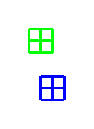
\begin{tikzpicture}[scale=0.15]
    \drawBinaryImage{7}{7}{imgMaxTreeDNodeOnlyRed}
    \draw[green, line width=1pt] (4,6) grid (6,4);
    \draw[blue, line width=1pt] (5,2) grid (7,0);
  \end{tikzpicture}
\end{lrbox}